documentclass{article}

\usepackage{tikz}
\usetikzlibrary{positioning}

\begin{document}

\begin{figure}[h]
  \centering
  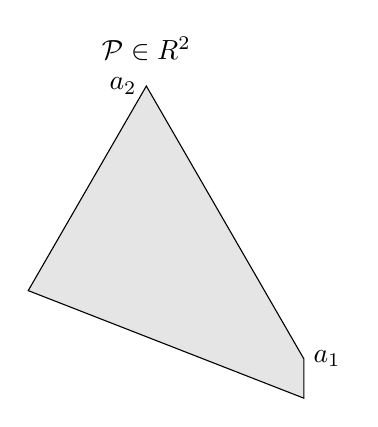
\begin{tikzpicture}[%
    myvector/.style={
      -latex,
      draw=black!50,
      line width=1pt,
      shorten >=3pt,
      shorten <=3pt,
      },
    mytext/.style={fill=white,font=\scriptsize,text depth=.7ex},
    ]
    \draw[fill=gray!20] 
        (0,0) coordinate(-bottom-left)
        --++(60:3cm) coordinate (-top-left) node[left]{$a_2$}
        --++(300:4cm) coordinate (-top-right) node[right]{$a_1$}
        --++(-90:.5cm) coordinate (-bottom-right)
        --cycle;
    \node[above=2mm] at (-top-left) {$\mathcal{P}\in\mathbb{R}^{2}$};
  \end{tikzpicture}
  
  \quad
  
  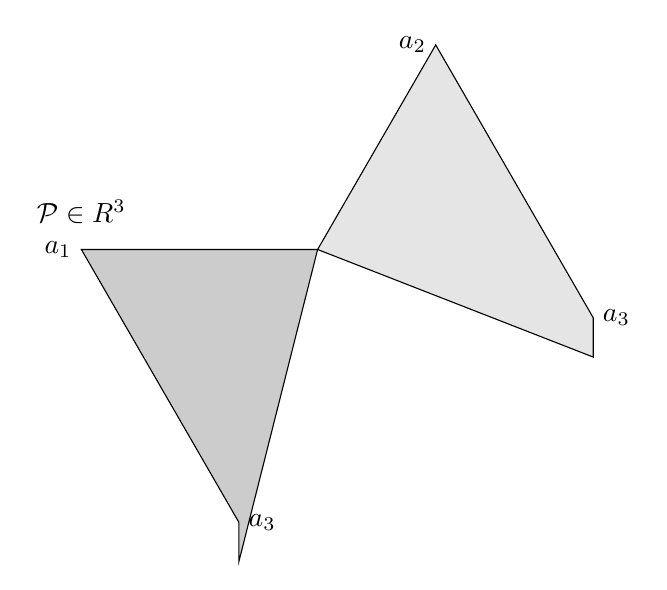
\begin{tikzpicture}[%
    myvector/.style={
      -latex,
      draw=black!50,
      line width=1pt,
      shorten >=3pt,
      shorten <=3pt,
      },
    mytext/.style={fill=white,font=\scriptsize,text depth=.7ex},
    ]
    \draw[fill=gray!20] 
        (0,0) coordinate(-bottom-left)
        --++(60:3cm) coordinate (-top-left) node[left]{$a_2$}
        --++(300:4cm) coordinate (-top-right) node[right]{$a_3$}
        --++(-90:.5cm) coordinate (-bottom-right)
        --cycle;
    \draw[fill=gray!40] 
        (0,0) coordinate(-bottom-left)
        --++(180:3cm) coordinate (-top-left) node[left]{$a_1$}
        --++(300:4cm) coordinate (-top-right) node[right]{$a_3$}
        --++(-90:.5cm) coordinate (-bottom-right)
        --cycle;
    \node[above=2mm] at (-top-left) {$\mathcal{P}\in\mathbb{R}^{3}$};
  \end{tikzpicture}
\end{figure}

\end{document}